\externaldocument{eval}

\chapter{Further Results}
\label{appendix:FurtherResults}
\markright{FurtherResults}

The real world implementation of this thesis available as open source software. The code can be found at \url{https://github.com/hias234/AustrianParliamentAnalyzer}. In the following chapter some screen shots of the web application and all relation graphs from the periods 20 to 25 are shown.

\section{Screenshots of the Web Application}

The start page shown in figure \ref{fig:start_page} shows an overview of the current period (mandate distribution, absence, ...) and gives the possibility to navigate to all other pages. The period analysis page shows statistics about a certain period. Figure \ref{fig:screenshot_period} shows the period analysis of period 24. The most absent clubs and politicians and the politicians with the most speeches are shown there. Figure \ref{fig:screenshot_politician} shows the politician analysis page for Sonja Ablinger. It shows basic personal data, the mandates held and politicians with similar and contrary attitudes.

\begin{figure}[h]
	\center
	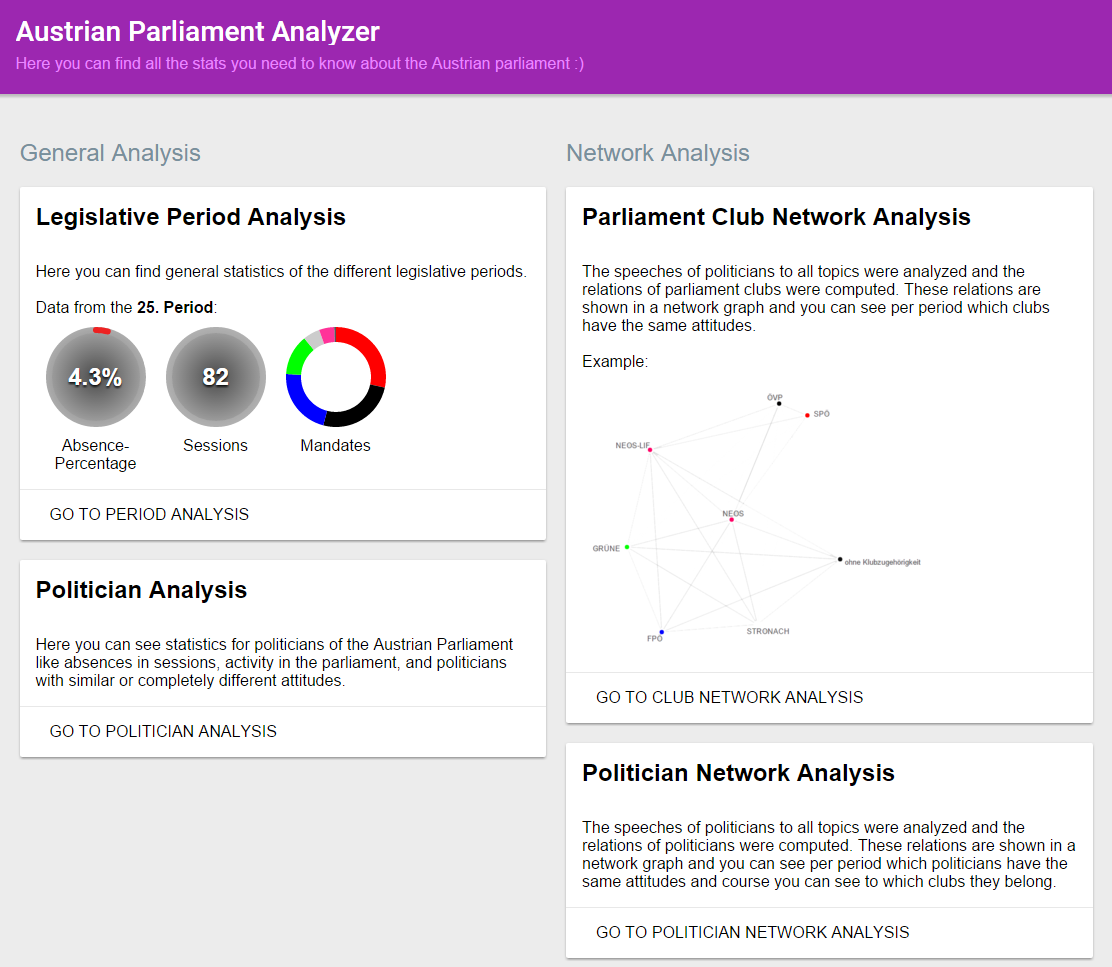
\includegraphics[width=0.85\textwidth]{imgs/result_start_page}
	\caption{Start Page of the Prototype Web Application}
	\label{fig:start_page}
\end{figure}

\begin{figure}[h!]
	\center
	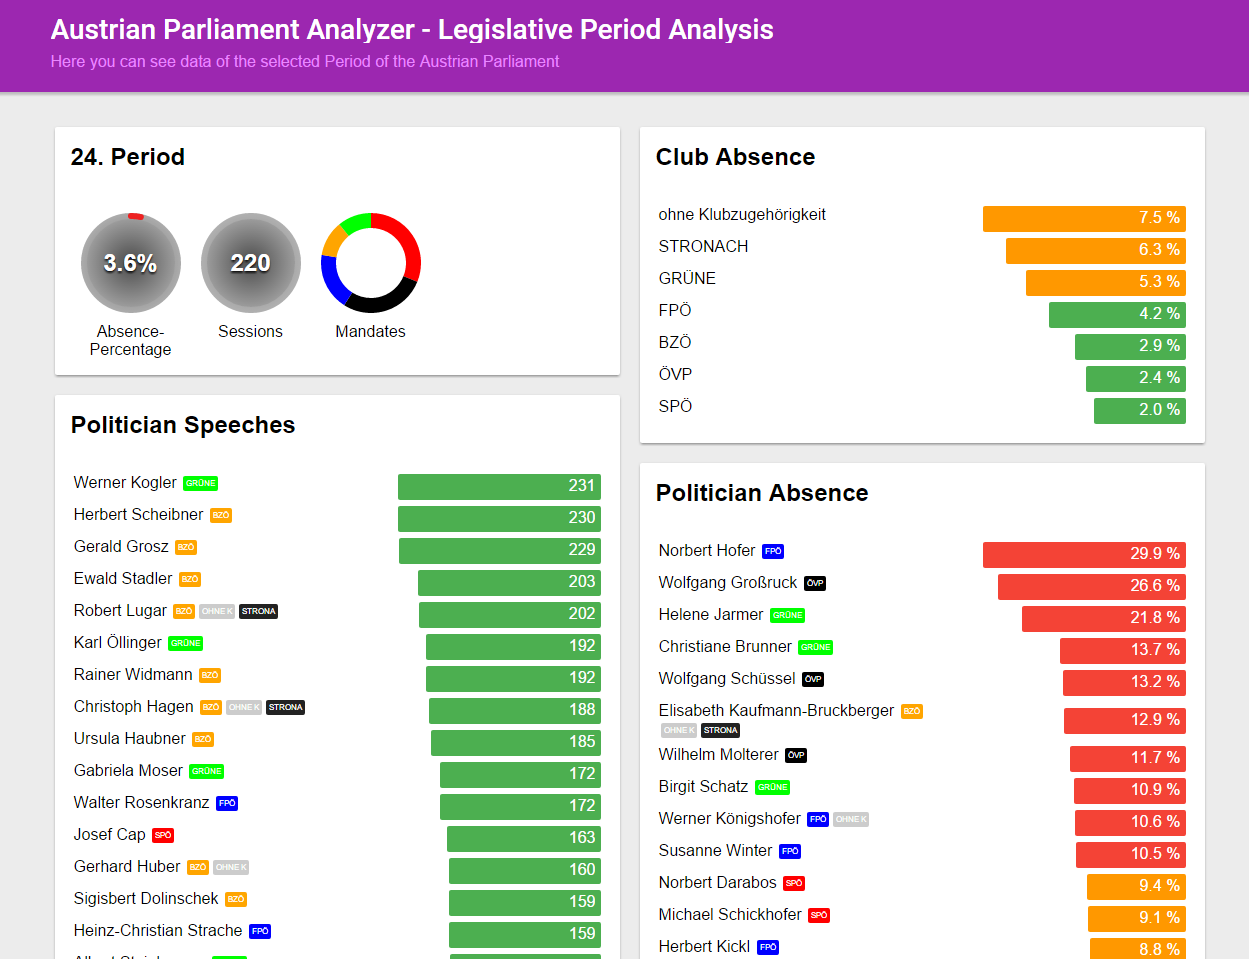
\includegraphics[width=0.85\textwidth]{imgs/screenshot_period}
	\caption{Period Analysis Page (Period 24)}
	\label{fig:screenshot_period}
\end{figure}

\begin{figure}[h!]
	\center
	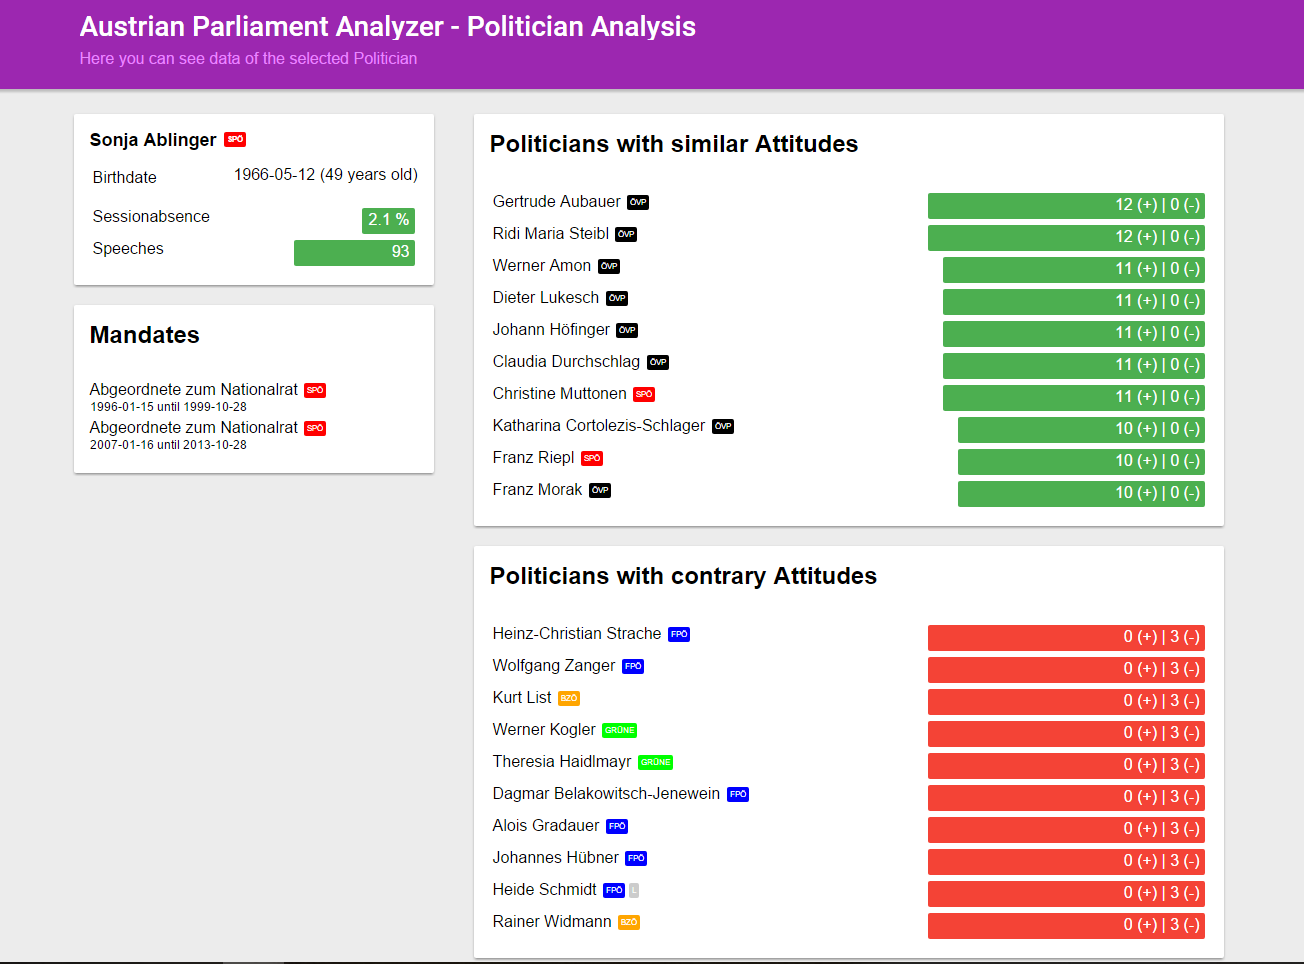
\includegraphics[width=0.85\textwidth]{imgs/screenshot_politician}
	\caption{Politician Analysis Page (Sonja Ablinger)}
	\label{fig:screenshot_politician}
\end{figure}

\pagebreak
\pagebreak

\section{Club Relation Graphs}

Figure \ref{fig:all_club_graphs} shows the club graphs for all legislative periods. As discussed in chapter \ref{chap:evaluation} government and opposition are highly distinct in each period.

\begin{figure}[h!]
	\center
	\setlength{\tabcolsep}{.26667em}
	\begin{tabular}{ c | c }
		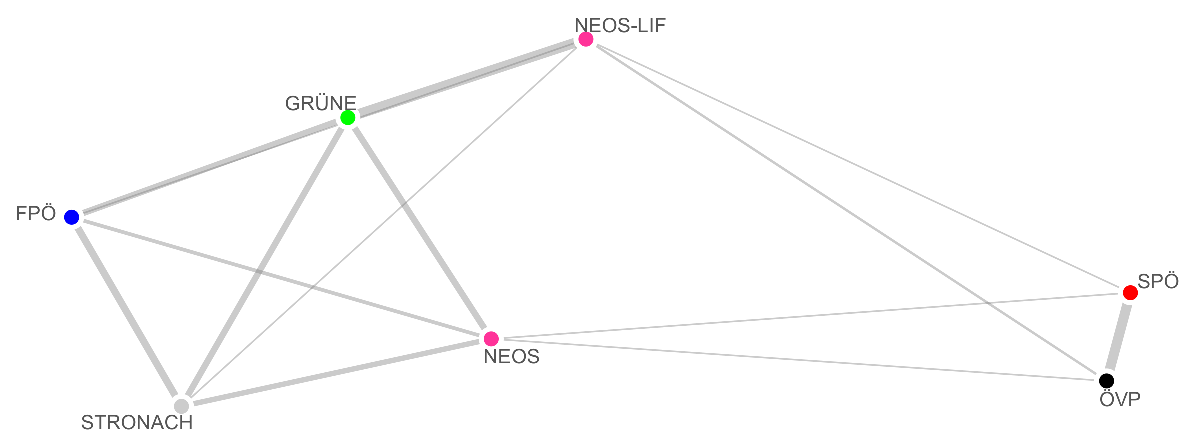
\includegraphics[width=0.48\textwidth]{imgs/graphs/club-graphs/horizontal/graph_25.eps}
		&
		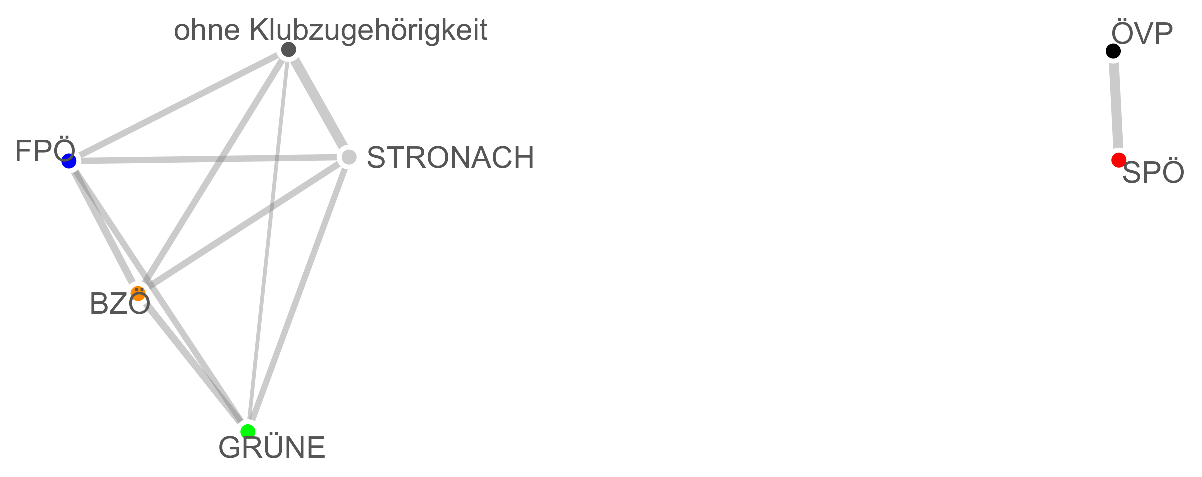
\includegraphics[width=0.48\textwidth]{imgs/graphs/club-graphs/horizontal/graph_24.eps}
		\\
		(a) 25. period
		&
		(b) 24. period
		
		\\
		\\
		\hline
		\\
		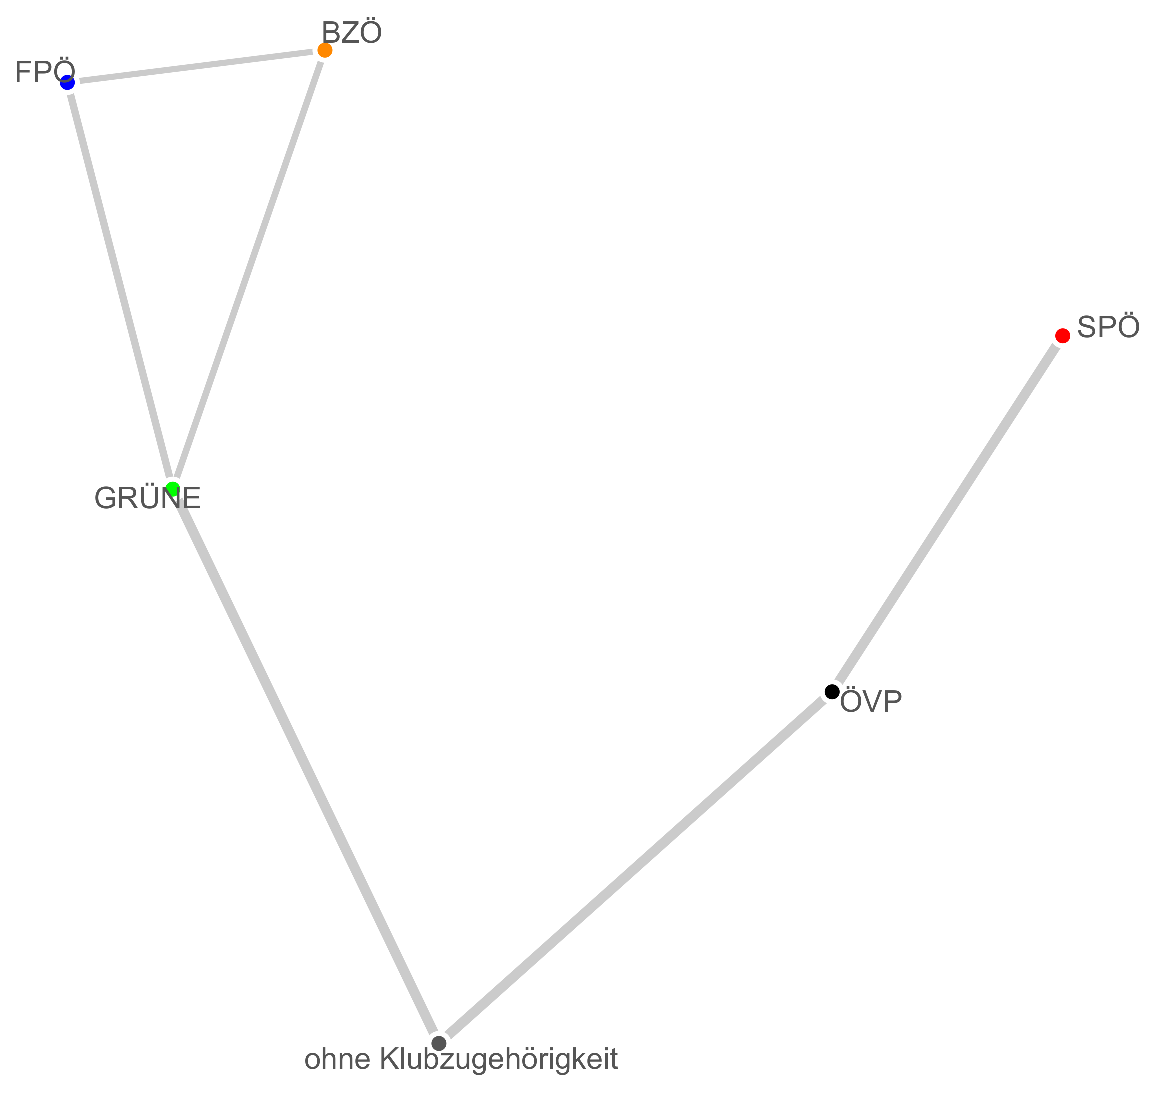
\includegraphics[width=0.48\textwidth]{imgs/graphs/club-graphs/horizontal/graph_23.eps}
		&
		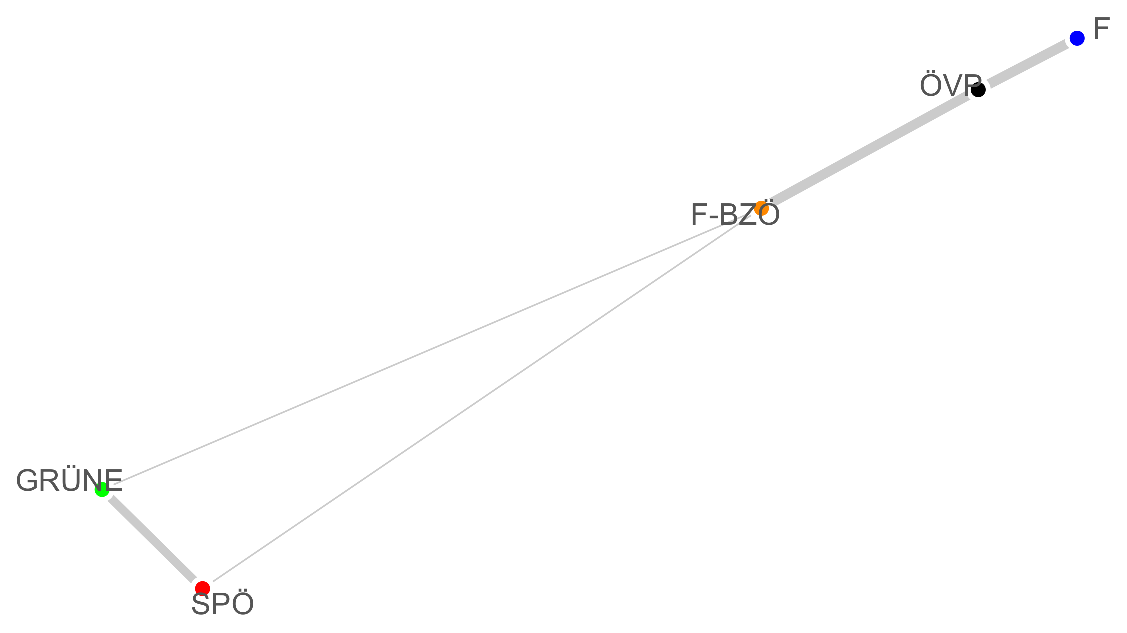
\includegraphics[width=0.48\textwidth]{imgs/graphs/club-graphs/horizontal/graph_22.eps}
		\\
		(c) 23. period
		&
		(d) 22. period
		\\
		\\
		\hline
		\\
		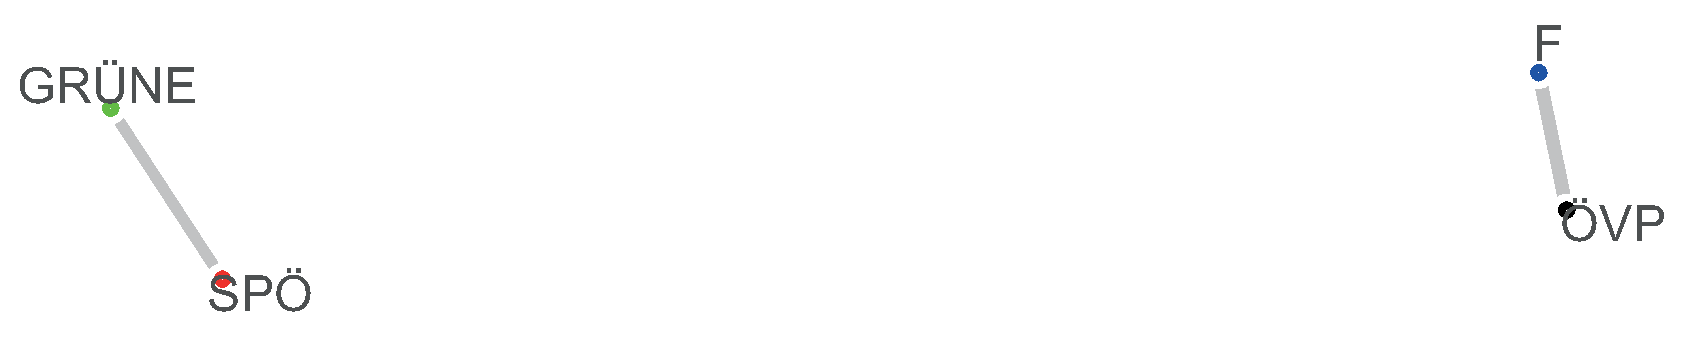
\includegraphics[width=0.48\textwidth]{imgs/graphs/club-graphs/horizontal/graph_21.eps}
		&
		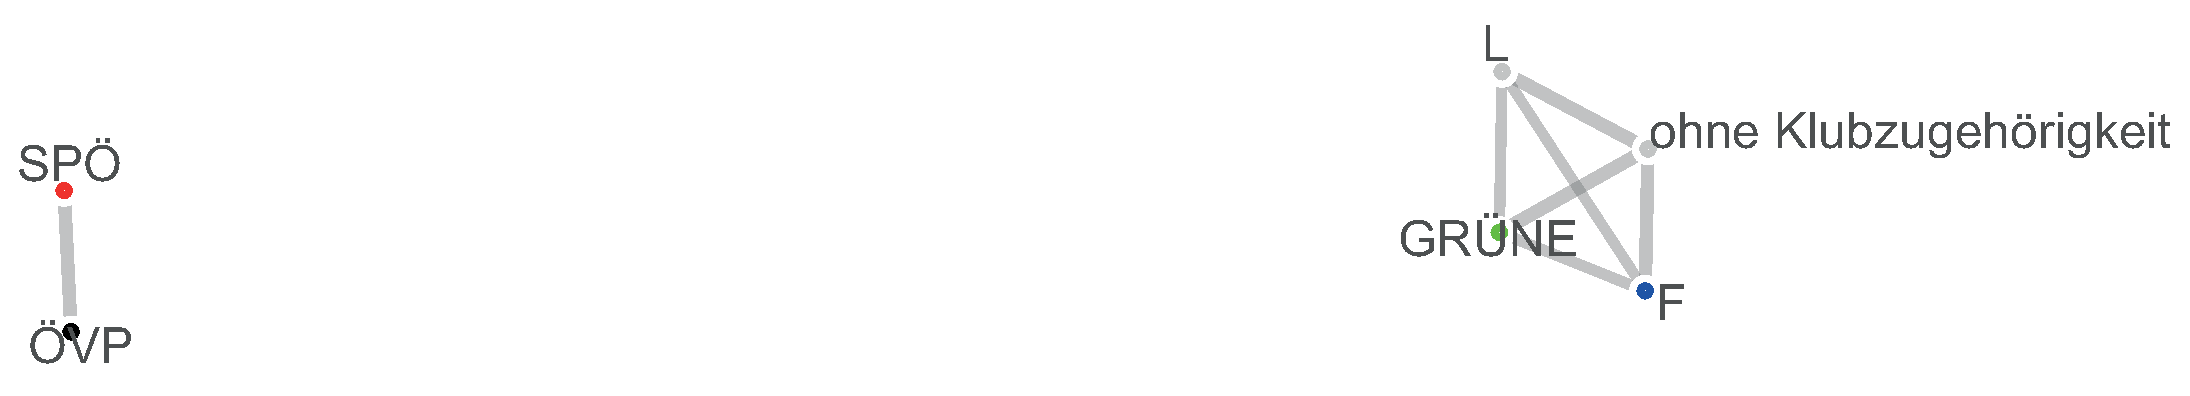
\includegraphics[width=0.48\textwidth]{imgs/graphs/club-graphs/horizontal/graph_20.eps}
		\\
		(e) 21. period
		&
		(f) 20. period	
		
	\end{tabular}

	\caption{Club Relation Graphs}
	\label{fig:all_club_graphs}
\end{figure}

\section{Politician Relation Graphs}

The figures \ref{fig:pol_graphs_20_21}, \ref{fig:pol_graphs_22_23} and \ref{fig:pol_graphs_24_25} show the politician relation graphs of the periods 20 to 25. The parties which were in government and opposition are listed in table \ref{table:gov_opp_parties}. The politician relation graphs got discussed in section \ref{sec:relations_pol}.

\begin{figure}
\center
\begin{tabular}{ c }
	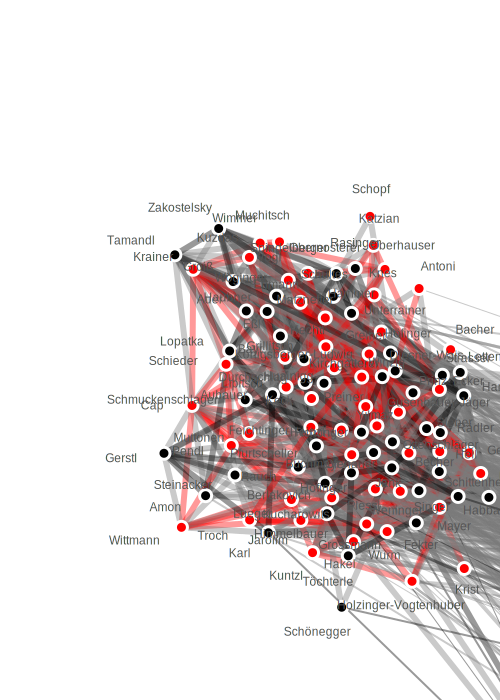
\includegraphics[width=0.85\textwidth]{imgs/graphs/politician-graphs/horizontal/graph_25.eps}
	\\
	(a) 25. Period
	\\
	\\
	\hline
	\\
	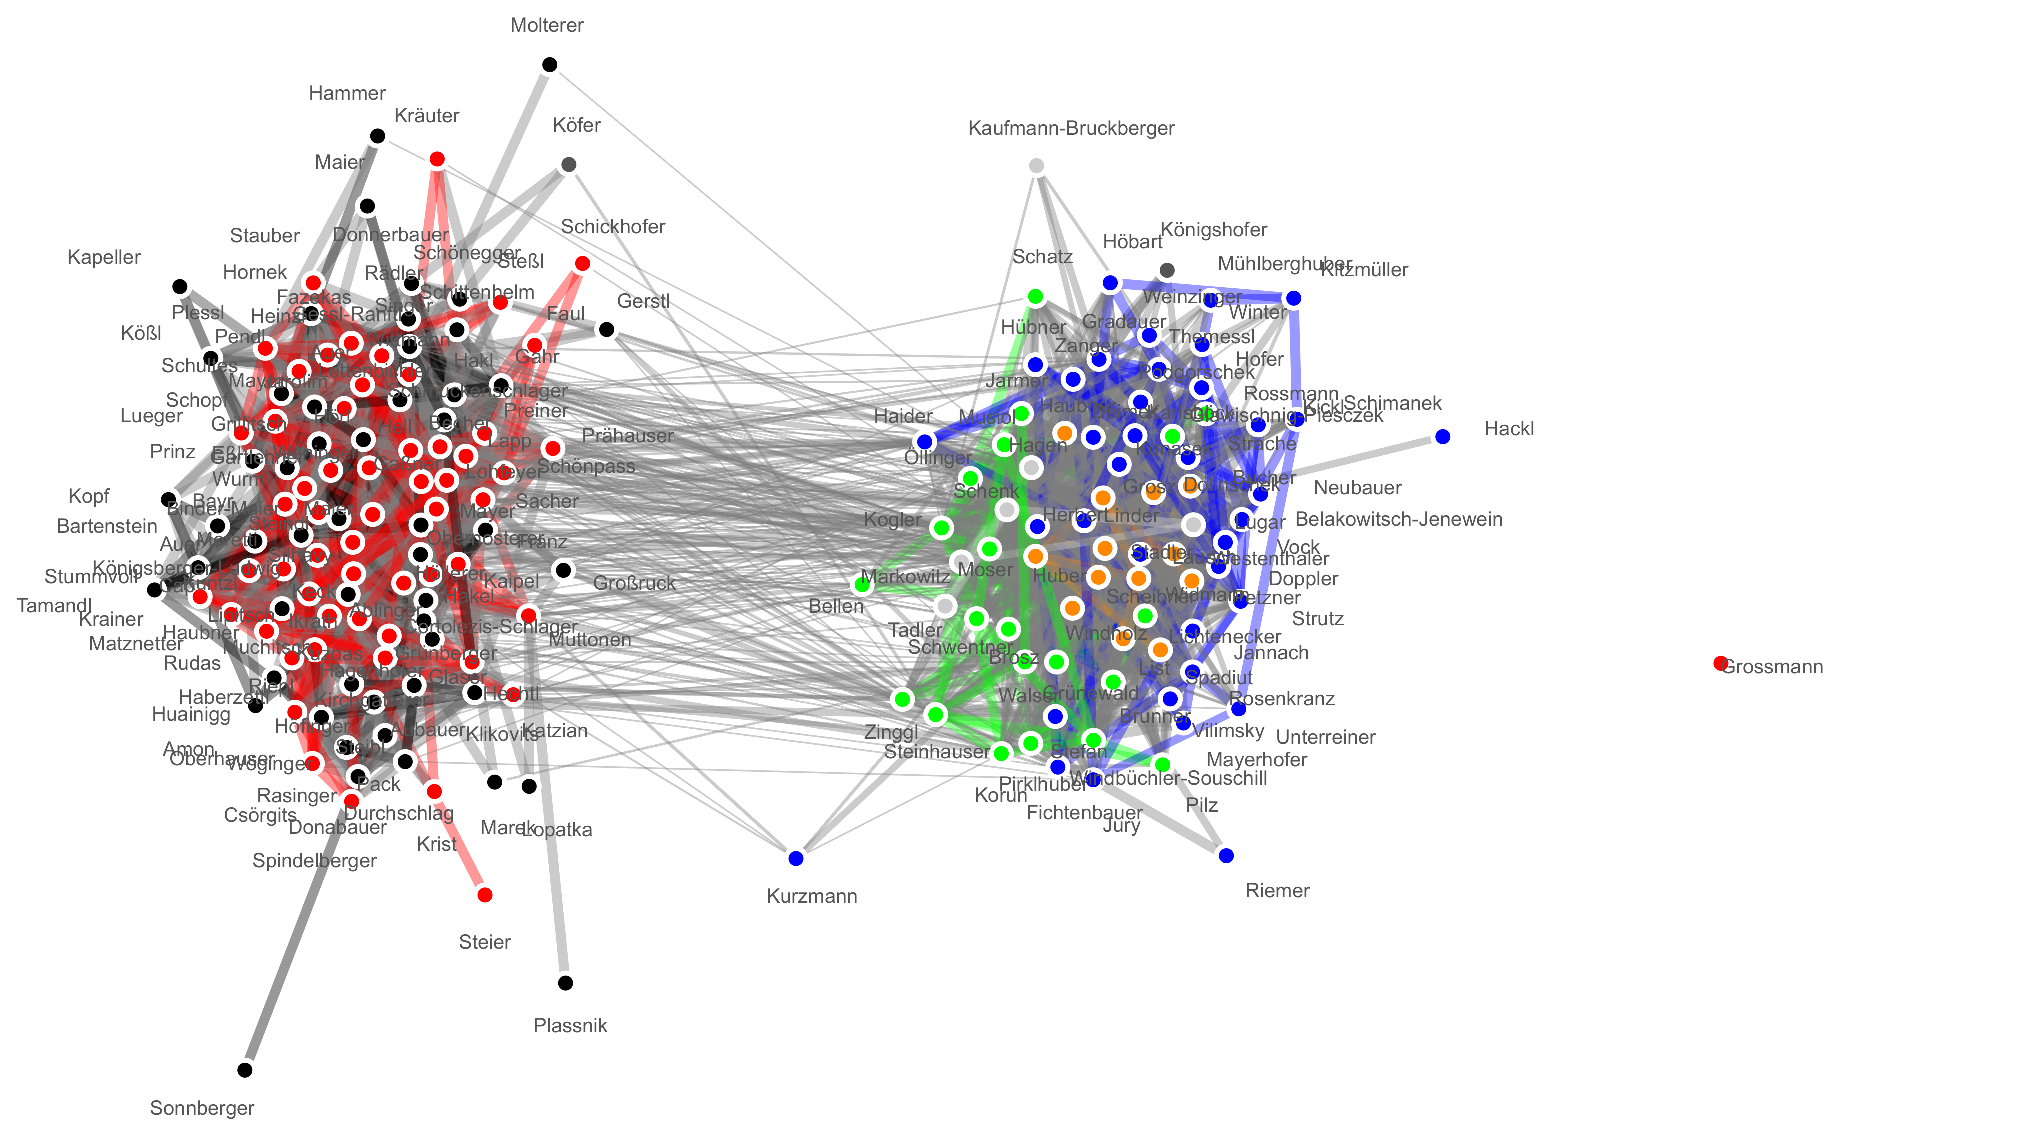
\includegraphics[width=0.85\textwidth]{imgs/graphs/politician-graphs/horizontal/graph_24.eps}
	\\
	(b) 24. Period
	
	%\\
	%\hline
	%\\
	%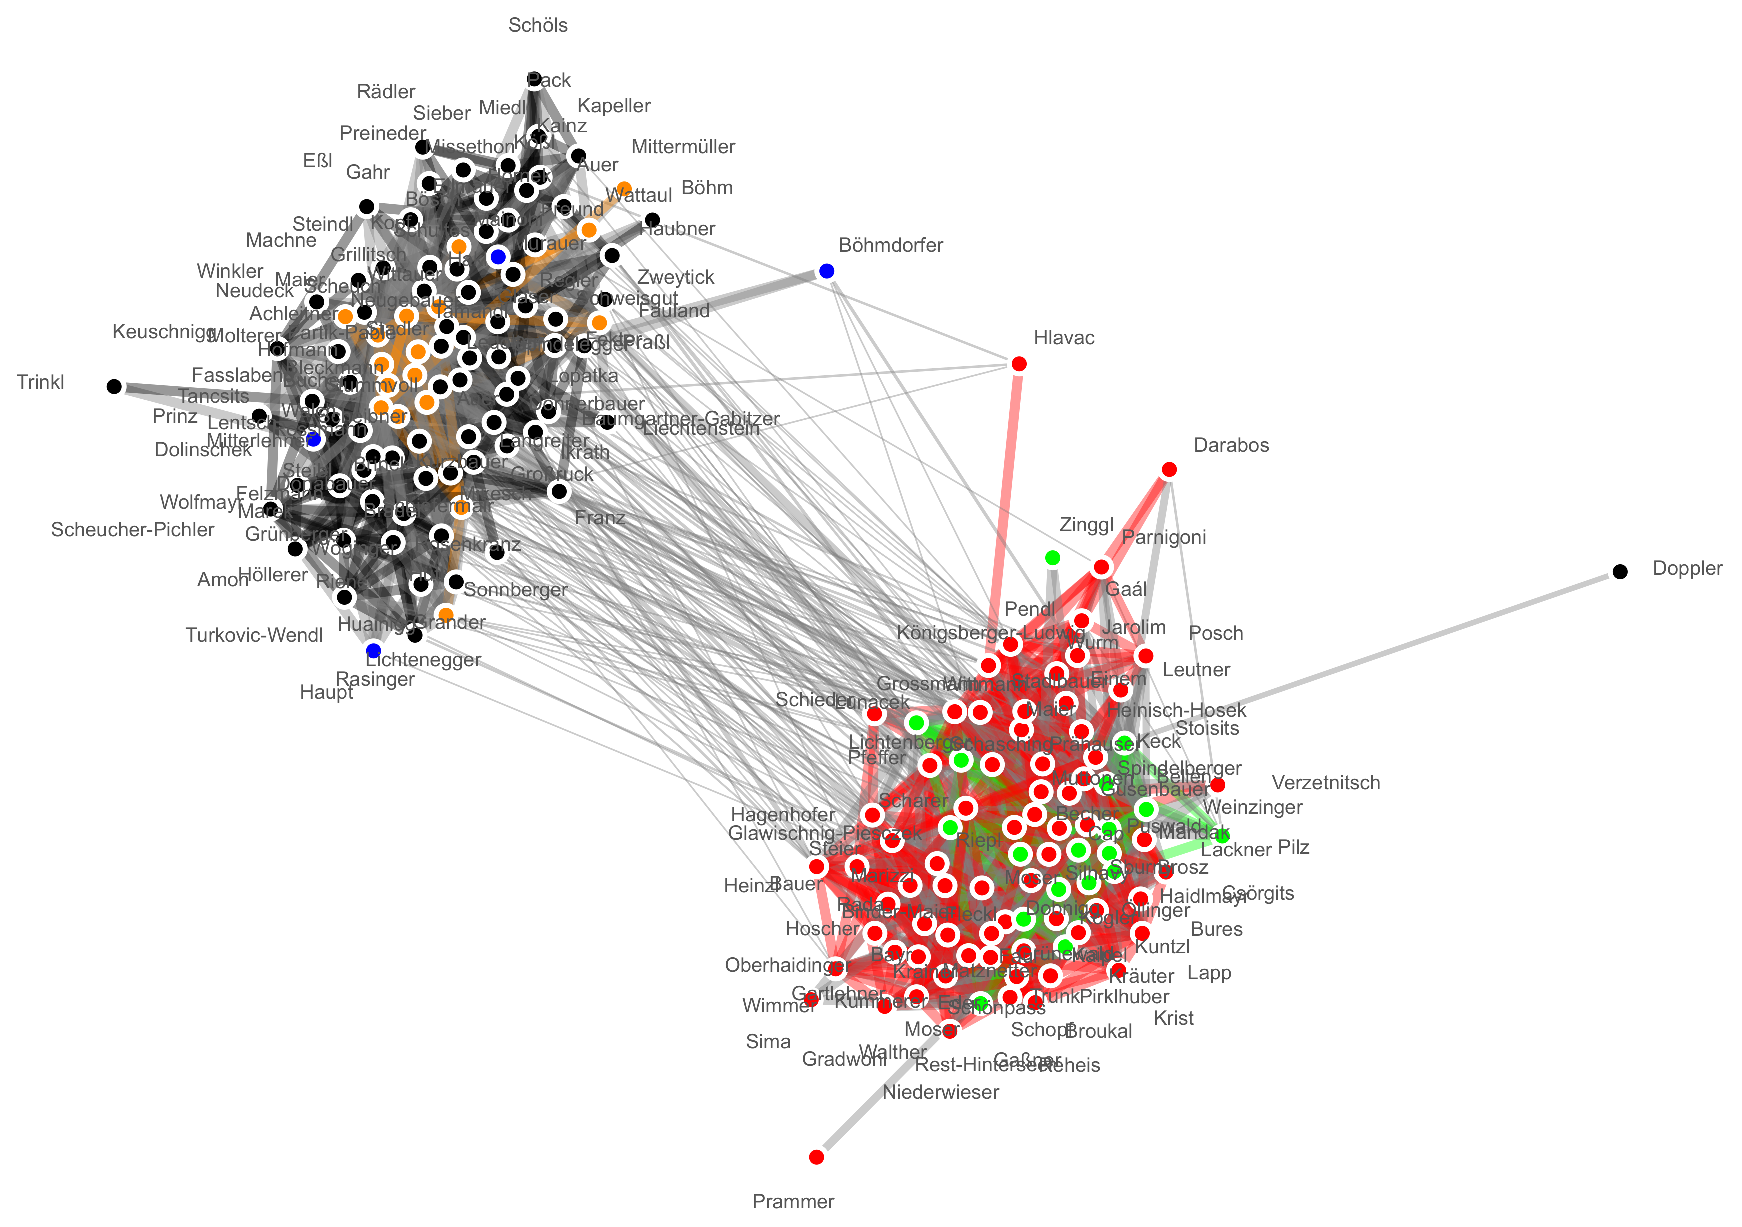
\includegraphics[width=0.85\textwidth]{imgs/graphs/politician-graphs/horizontal/graph_22.eps}
	%\\
	%(b) 22. Period
\end{tabular}
	
	
	\caption{Politician Relation Graphs - Periods 24 and 25}
	\label{fig:pol_graphs_24_25}
\end{figure}

\begin{figure}
\center
\begin{tabular}{ c }
	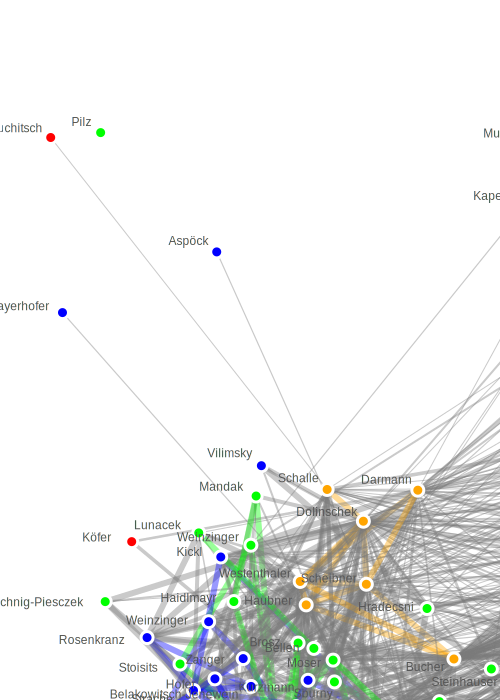
\includegraphics[width=0.85\textwidth]{imgs/graphs/politician-graphs/horizontal/graph_23.eps}
	\\
	(c) 23. Period
	\\
	
	\\
	\hline
	\\
	\\ 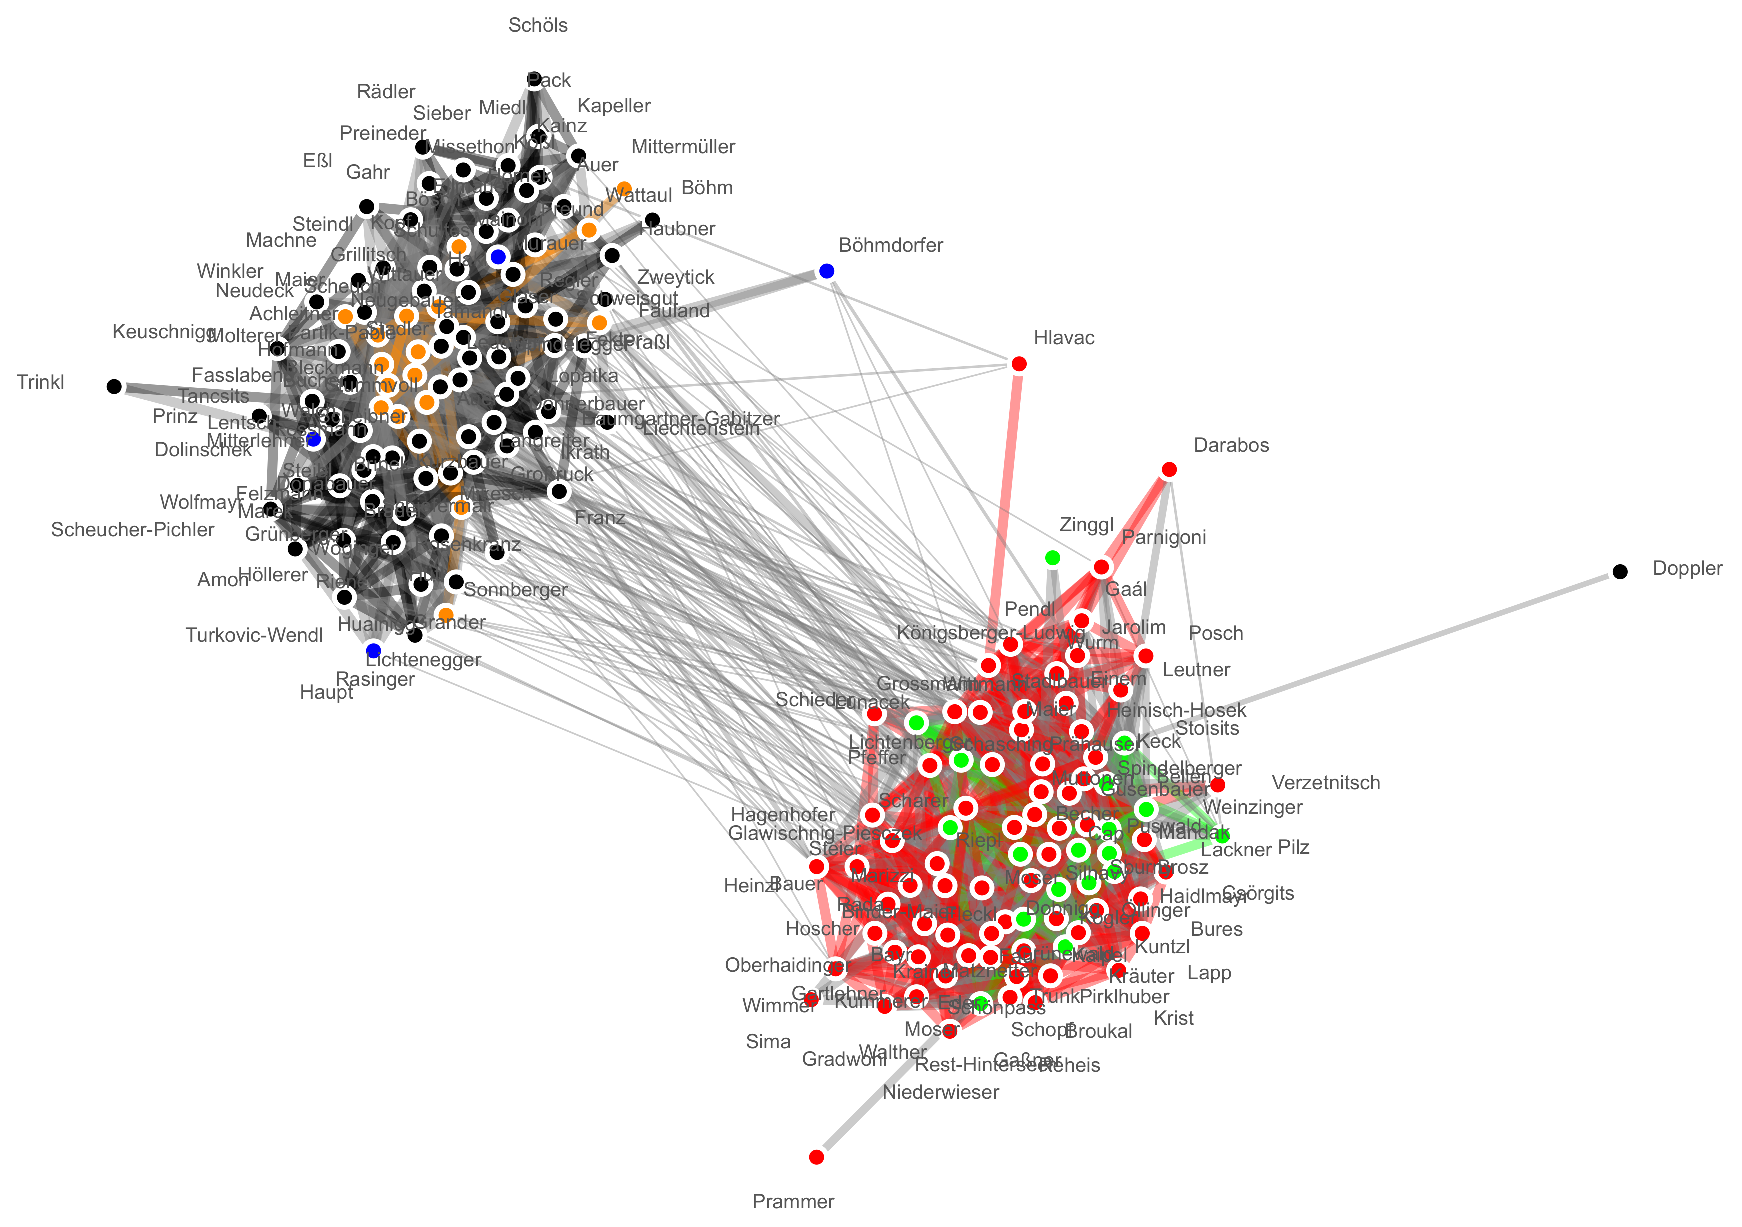
\includegraphics[width=0.85\textwidth]{imgs/graphs/politician-graphs/horizontal/graph_22.eps}
	\\
	(d) 22. Period
	
\end{tabular}
	
	
	\caption{Politician Relation Graphs - Periods 22 and 23}
	\label{fig:pol_graphs_22_23}
\end{figure}

\begin{figure}
\center
\begin{tabular}{ c }
	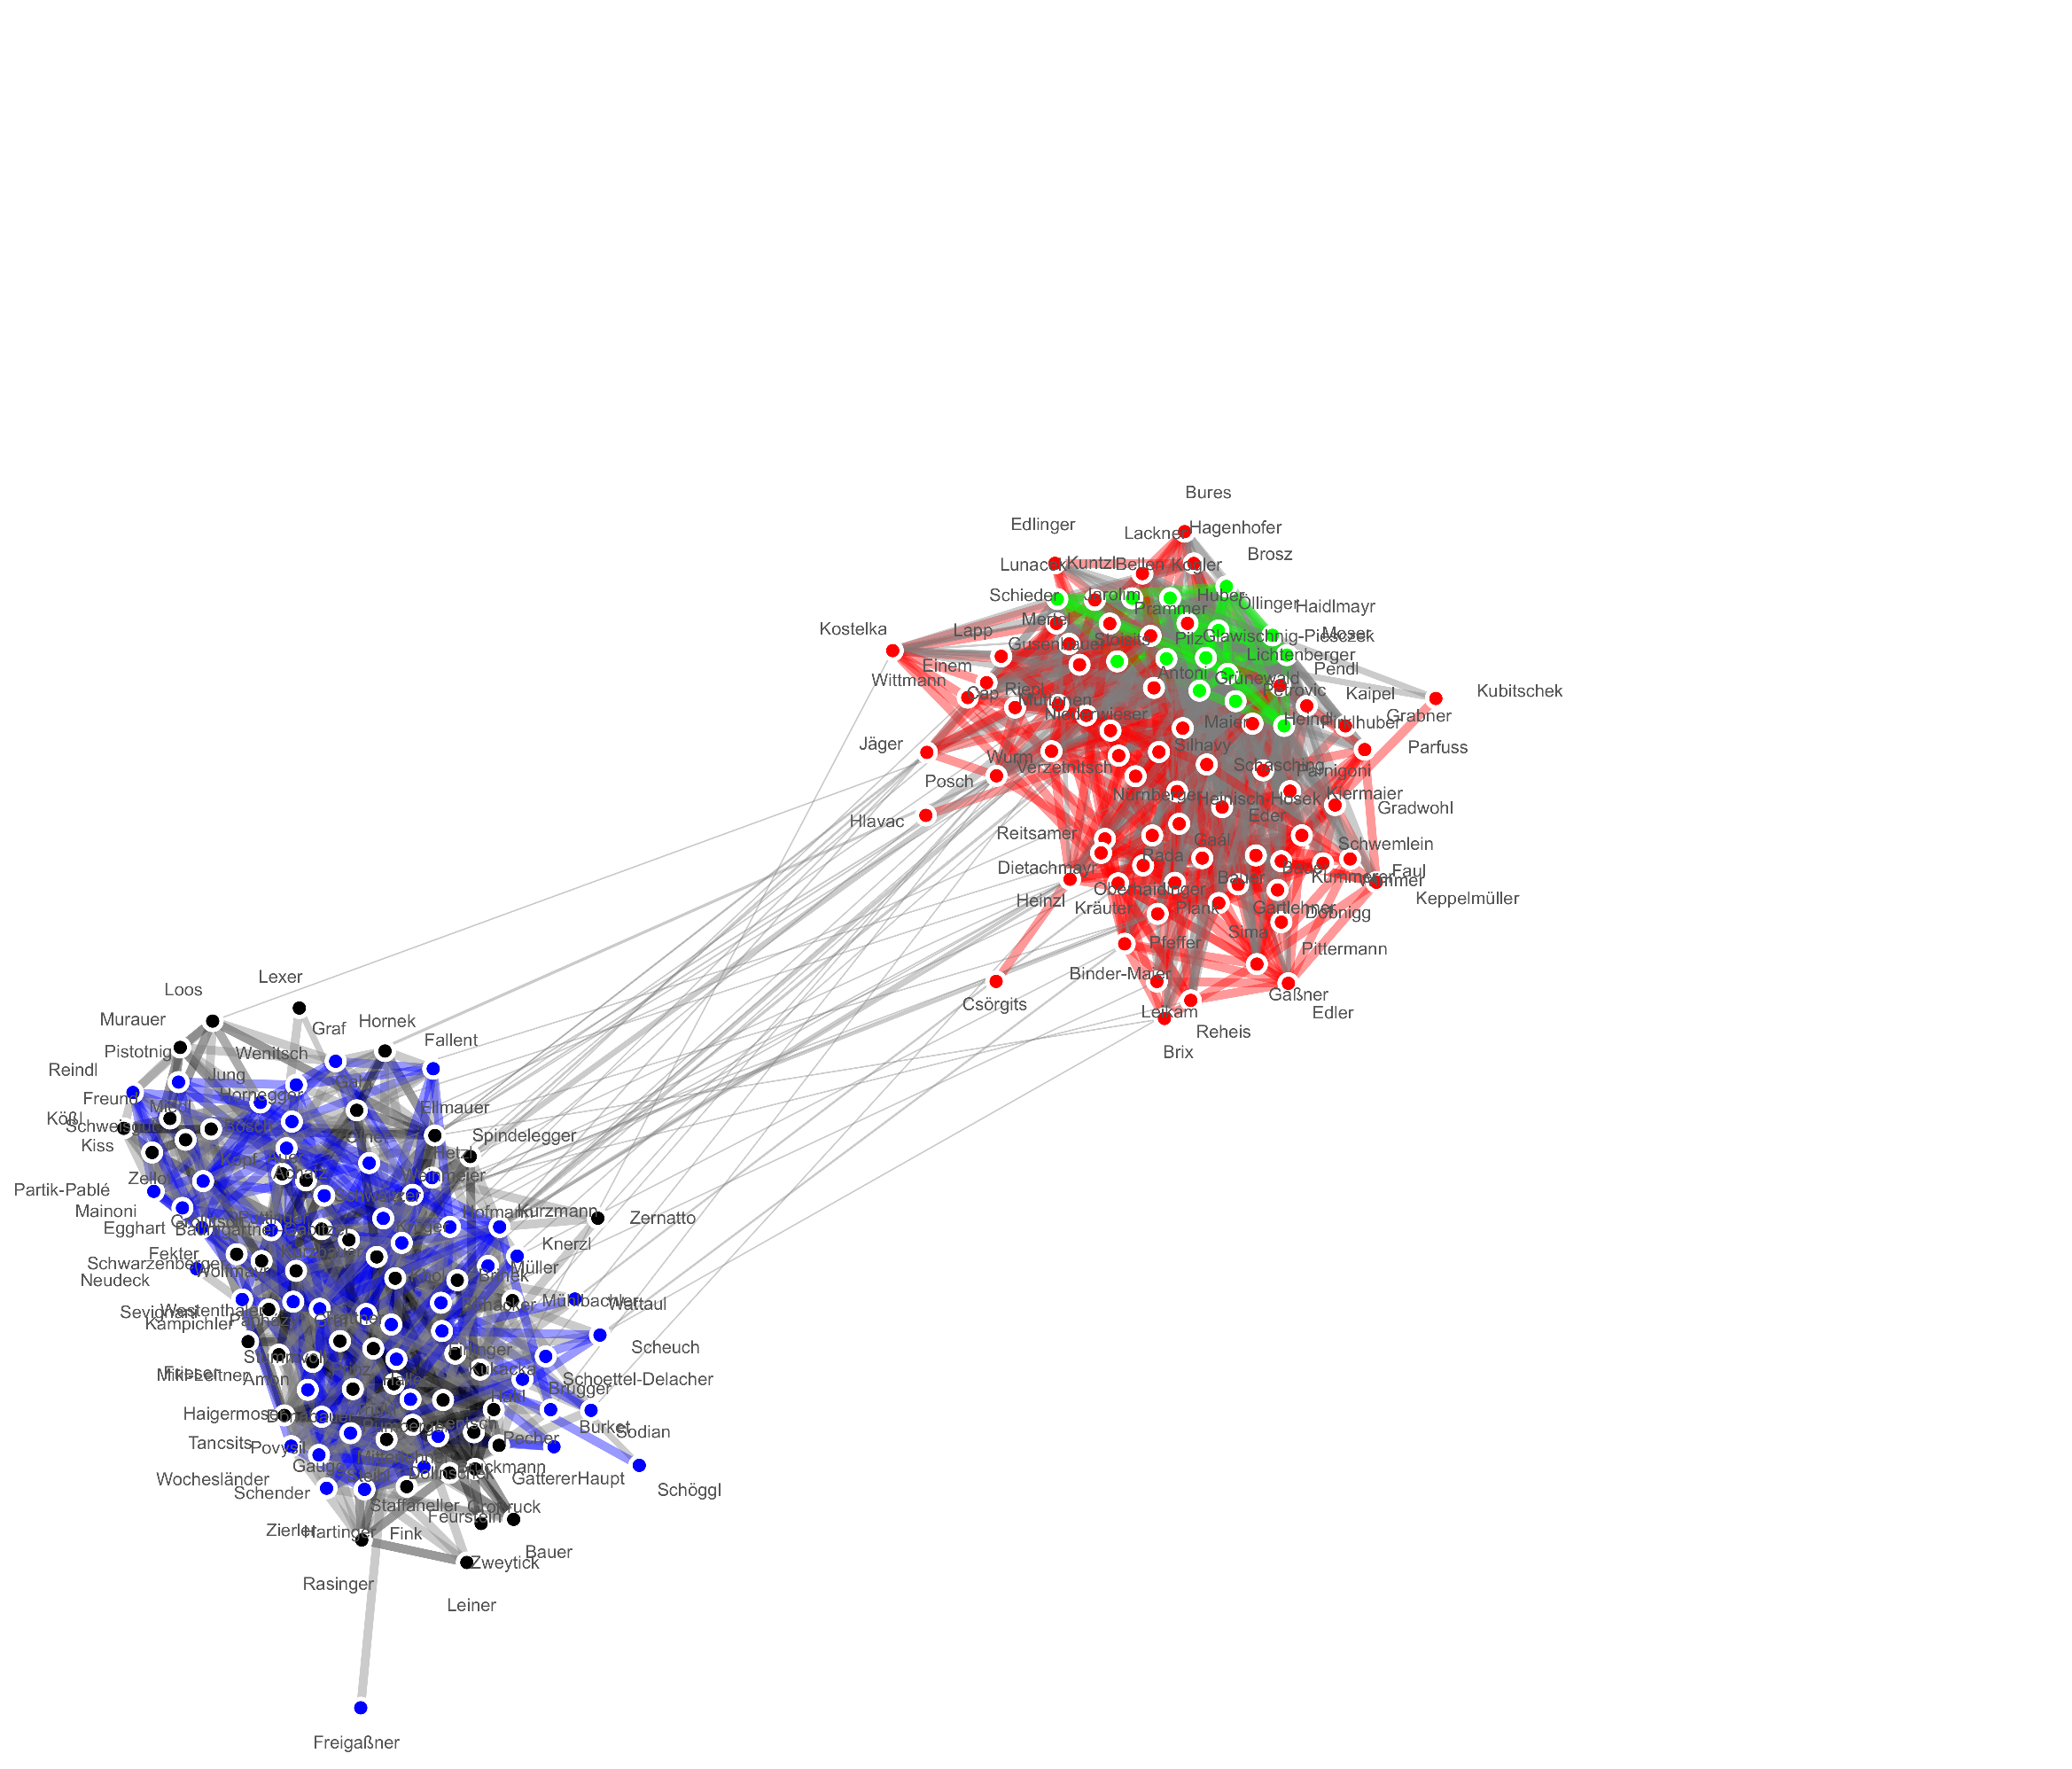
\includegraphics[width=0.85\textwidth]{imgs/graphs/politician-graphs/horizontal/graph_21.eps}
	\\
	(e) 21. Period
	\\
	
	\\
	\hline
	\\
	\\ 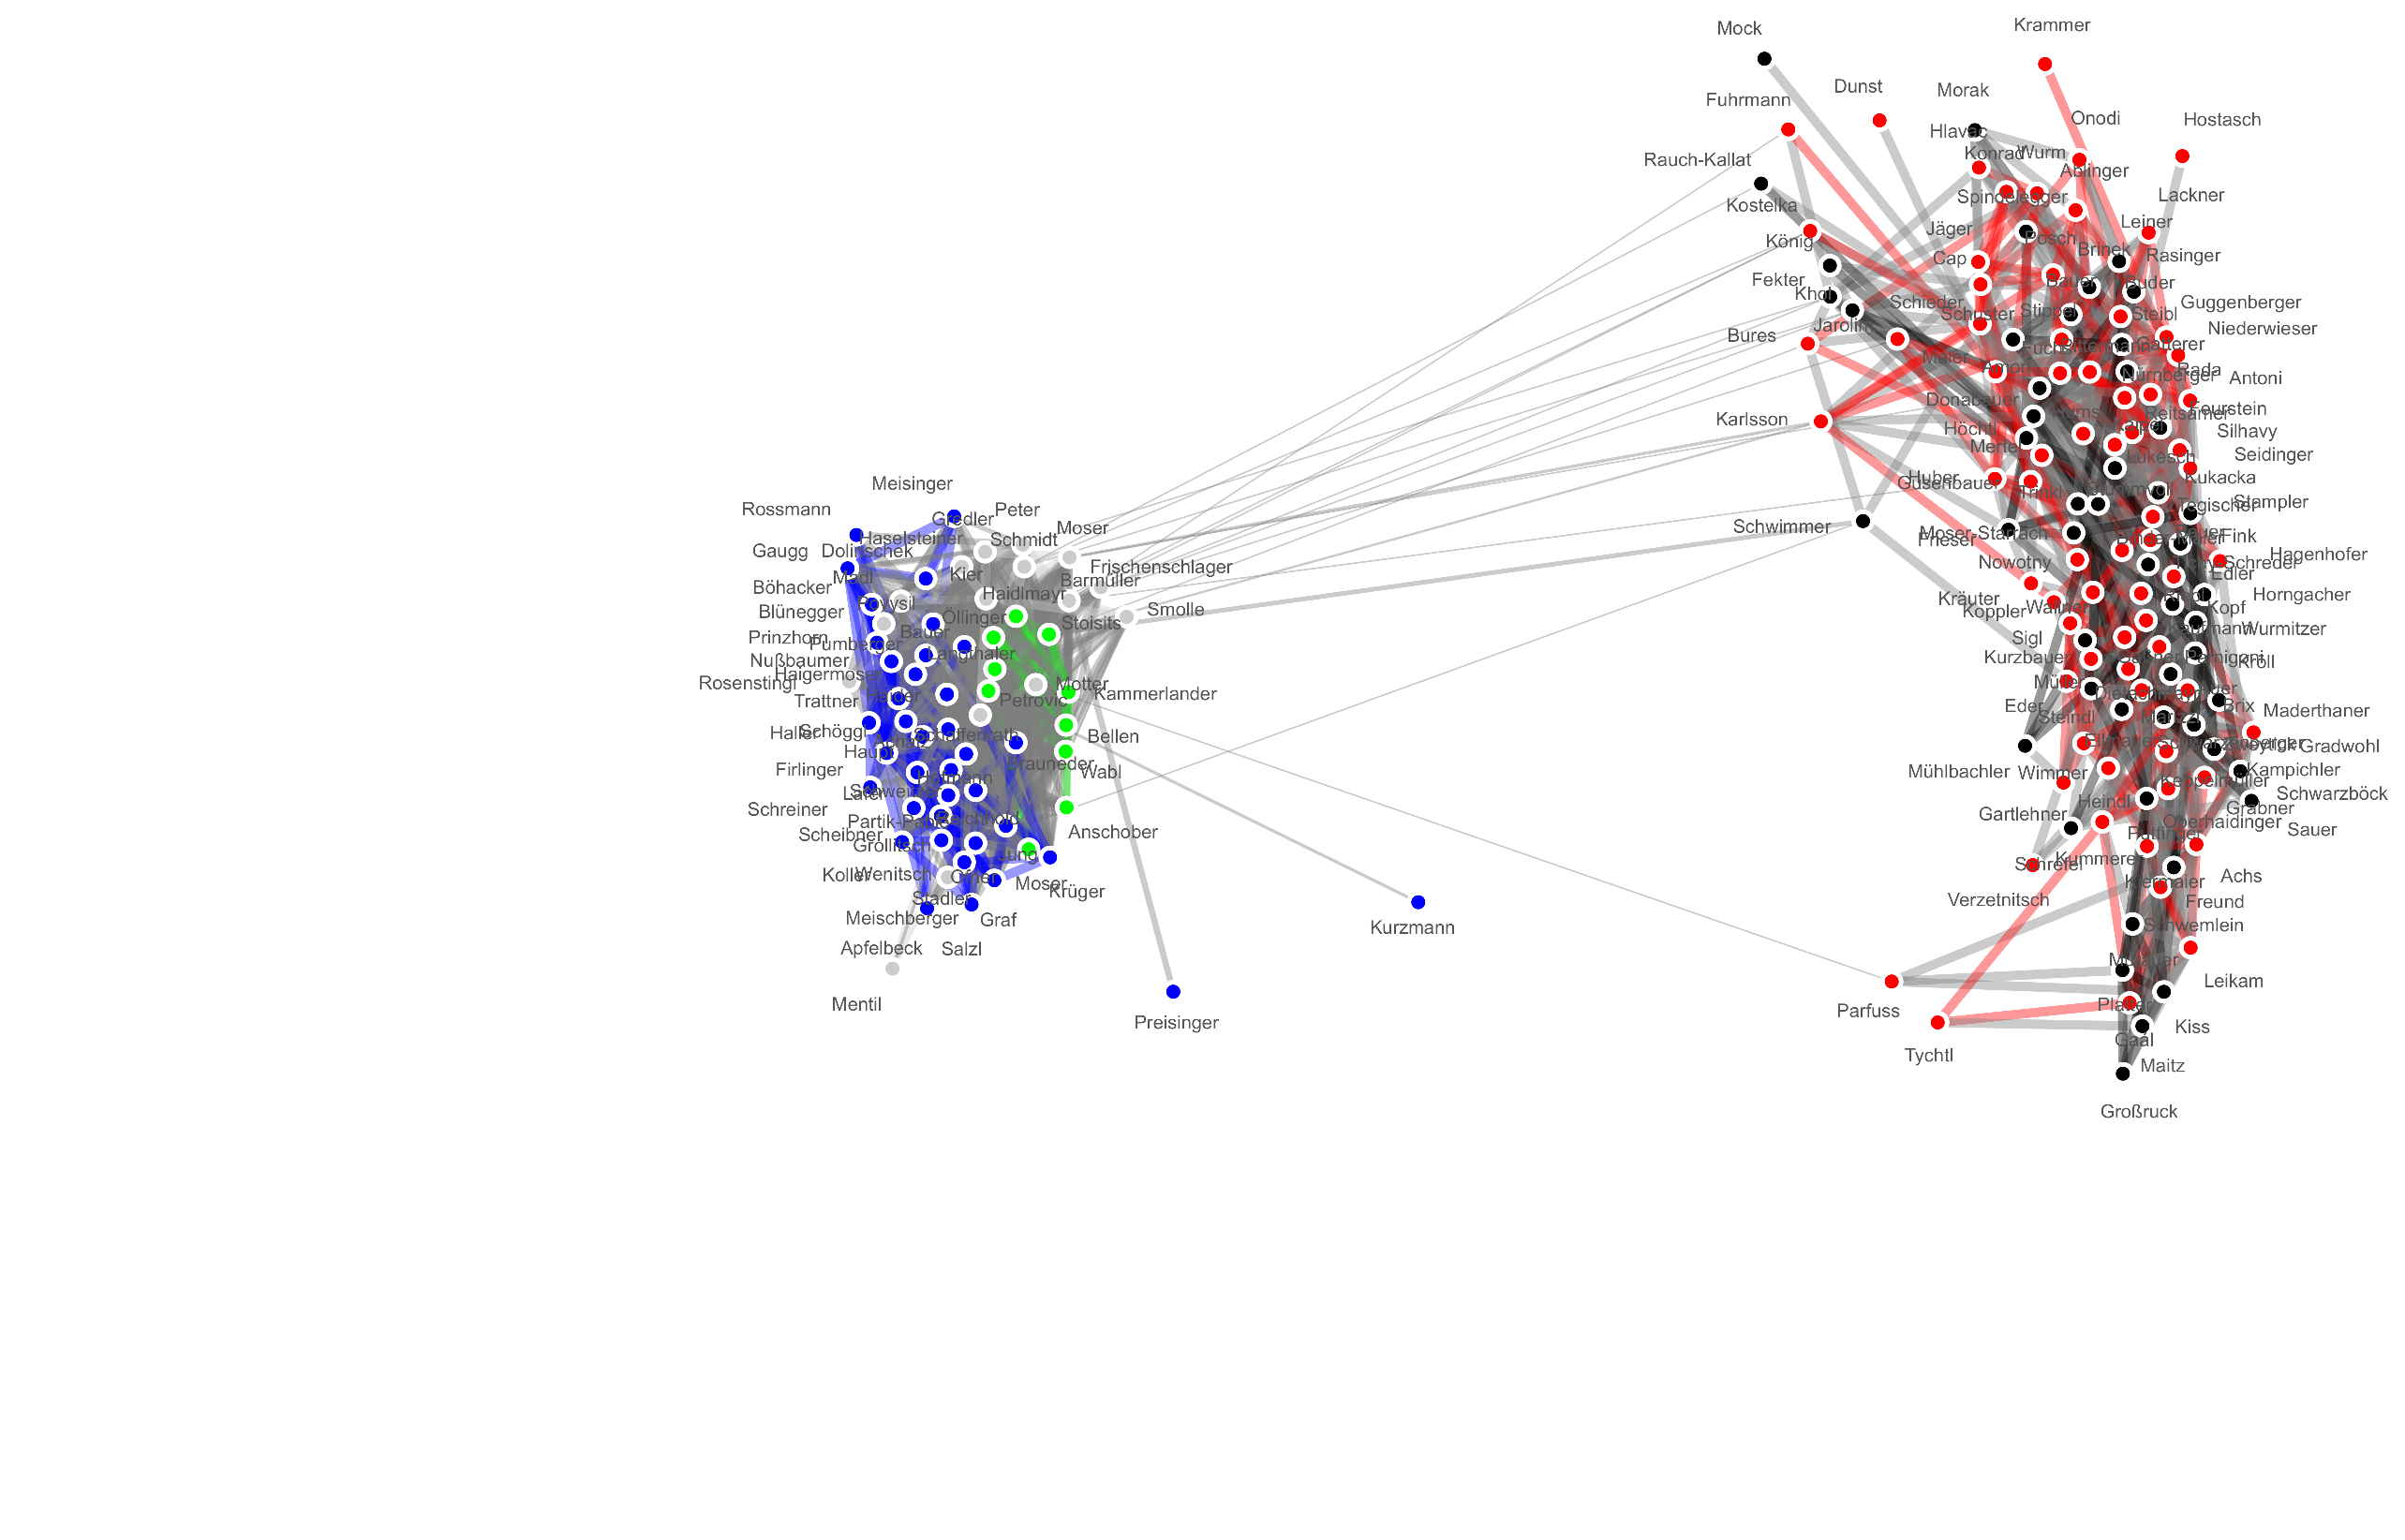
\includegraphics[width=0.85\textwidth]{imgs/graphs/politician-graphs/horizontal/graph_20.eps}
	\\
	(f) 20. Period
	
\end{tabular}
	
	
	\caption{Politician Relation Graphs - Periods 20 and 21}
	\label{fig:pol_graphs_20_21}
\end{figure}